\documentclass[12pt]{article}
\usepackage{graphicx}
\usepackage{float}

\title{Accurate calculation of the Earth Pressure using numerical integration}

\author{Rupak Kadel}

\begin{document}

\maketitle

\begin{abstract}
In this work we calculated the pressure inside the Earth as a function of the distance from the center of the Earth. We also calculated the pressure at the center of the earth which was approximately 364 GPa. It is almost equal to the realistic value which is around 360 Gpa. We estimated the pressure inside the earth using two different models of the earth. In the first model, we kept uniform density throughout the earth which resulted to the value of the pressure at the center that was lower by the factor of 2. We chose the Preliminary Reference Earth Model (PREM) as the second model of the Earth and calculated the value of density as a function of distance to the center of the earth. As a result,we obtained more realistic value for the pressure at the center of the earth. We also estimated the rotational inertia of Earth which was found to be $8.02 \times 10^{37} kgm^{2}$ which is almost equal to its realistic value.
\end{abstract}

\section{Introduction}
The inside structure of the Earth is layered in several spherical shells. Each layer has different chemical and physical properties due to which there is variation in the density of the earth. As we go deeper inside the earth, the density of each layer increases. The inner core is the most dense layer whereas the oceanic crust is the least dense layer of the earth. We have used the Preliminary Reference Earth Model, which was developed by Adam M. Dziewonski and Don L. Anderson, for this project. This model satisfies the guidelines that are set by the Standard Earth Model Committee. We used the equations for the density as a function of distance to the center of the earth from this model which resulted to almost accurate values for the density. The pressure inside the earth depends on the density and the mass enclosed as a function of distance to the center of the earth.

So, in order to find the pressure inside the earth, we considered a small element of mass 'm' inside the earth at a distance 'r' from the center of the earth. Let the height of this element be 'dr'. Since the object does not move, the net force acting on it is equal to zero. The pressure at the bottom of the object (at the distance 'r') is greater than the pressure at the distance 'r + dr'.  


\begin{figure}[H]
\centering
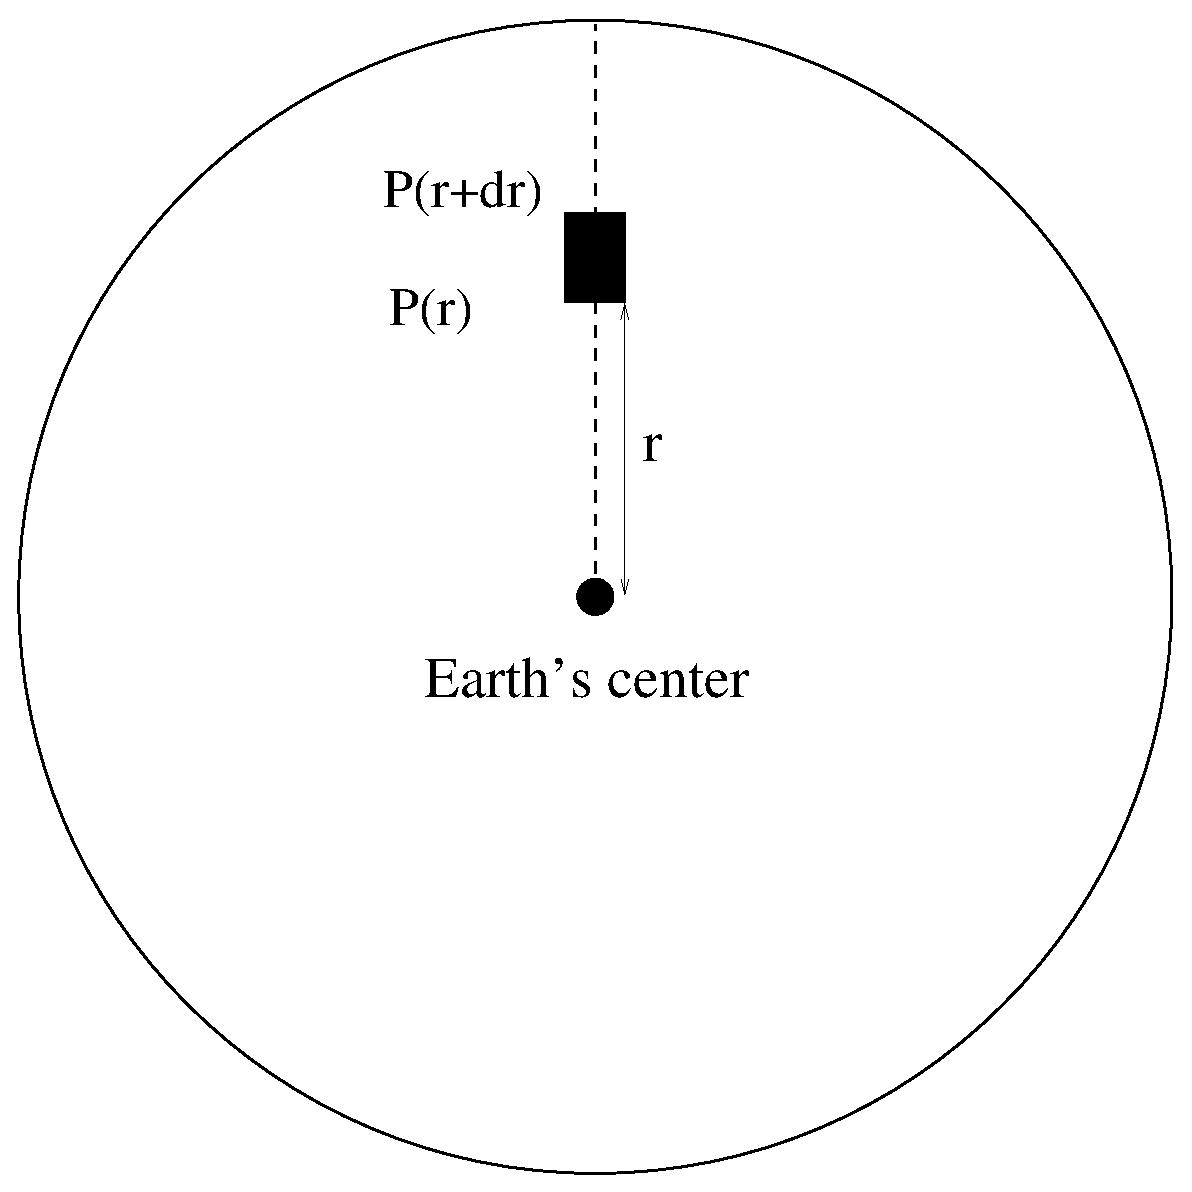
\includegraphics[width=0.5\textwidth]{earth_pressure.eps}\caption{A small element of mass 'm' at the distance 'r' from the center of the earth.}
\end{figure}

\section{Theory outlines}
The object experiences certain force due to the pressure gradient which can be written as:
\begin{equation}
F_P = [P(r) - P(r+dr)]*A
\end{equation}
It also experiences a force due to the gravitation and it can be represented as:
\begin{equation}
F_G = \frac{GMm}{r^2}
\end{equation}
where G,M,m and r are the Gravitational Constant, Mass enclosed by the object, mass of the object and the distance from the center of the earth respectively. 

Since the object does not move, the force due to pressure gradient must be equal to the gravitational force.
\begin{equation}
F_G = F_P,
\end{equation}

\begin{figure}[H]
\centering
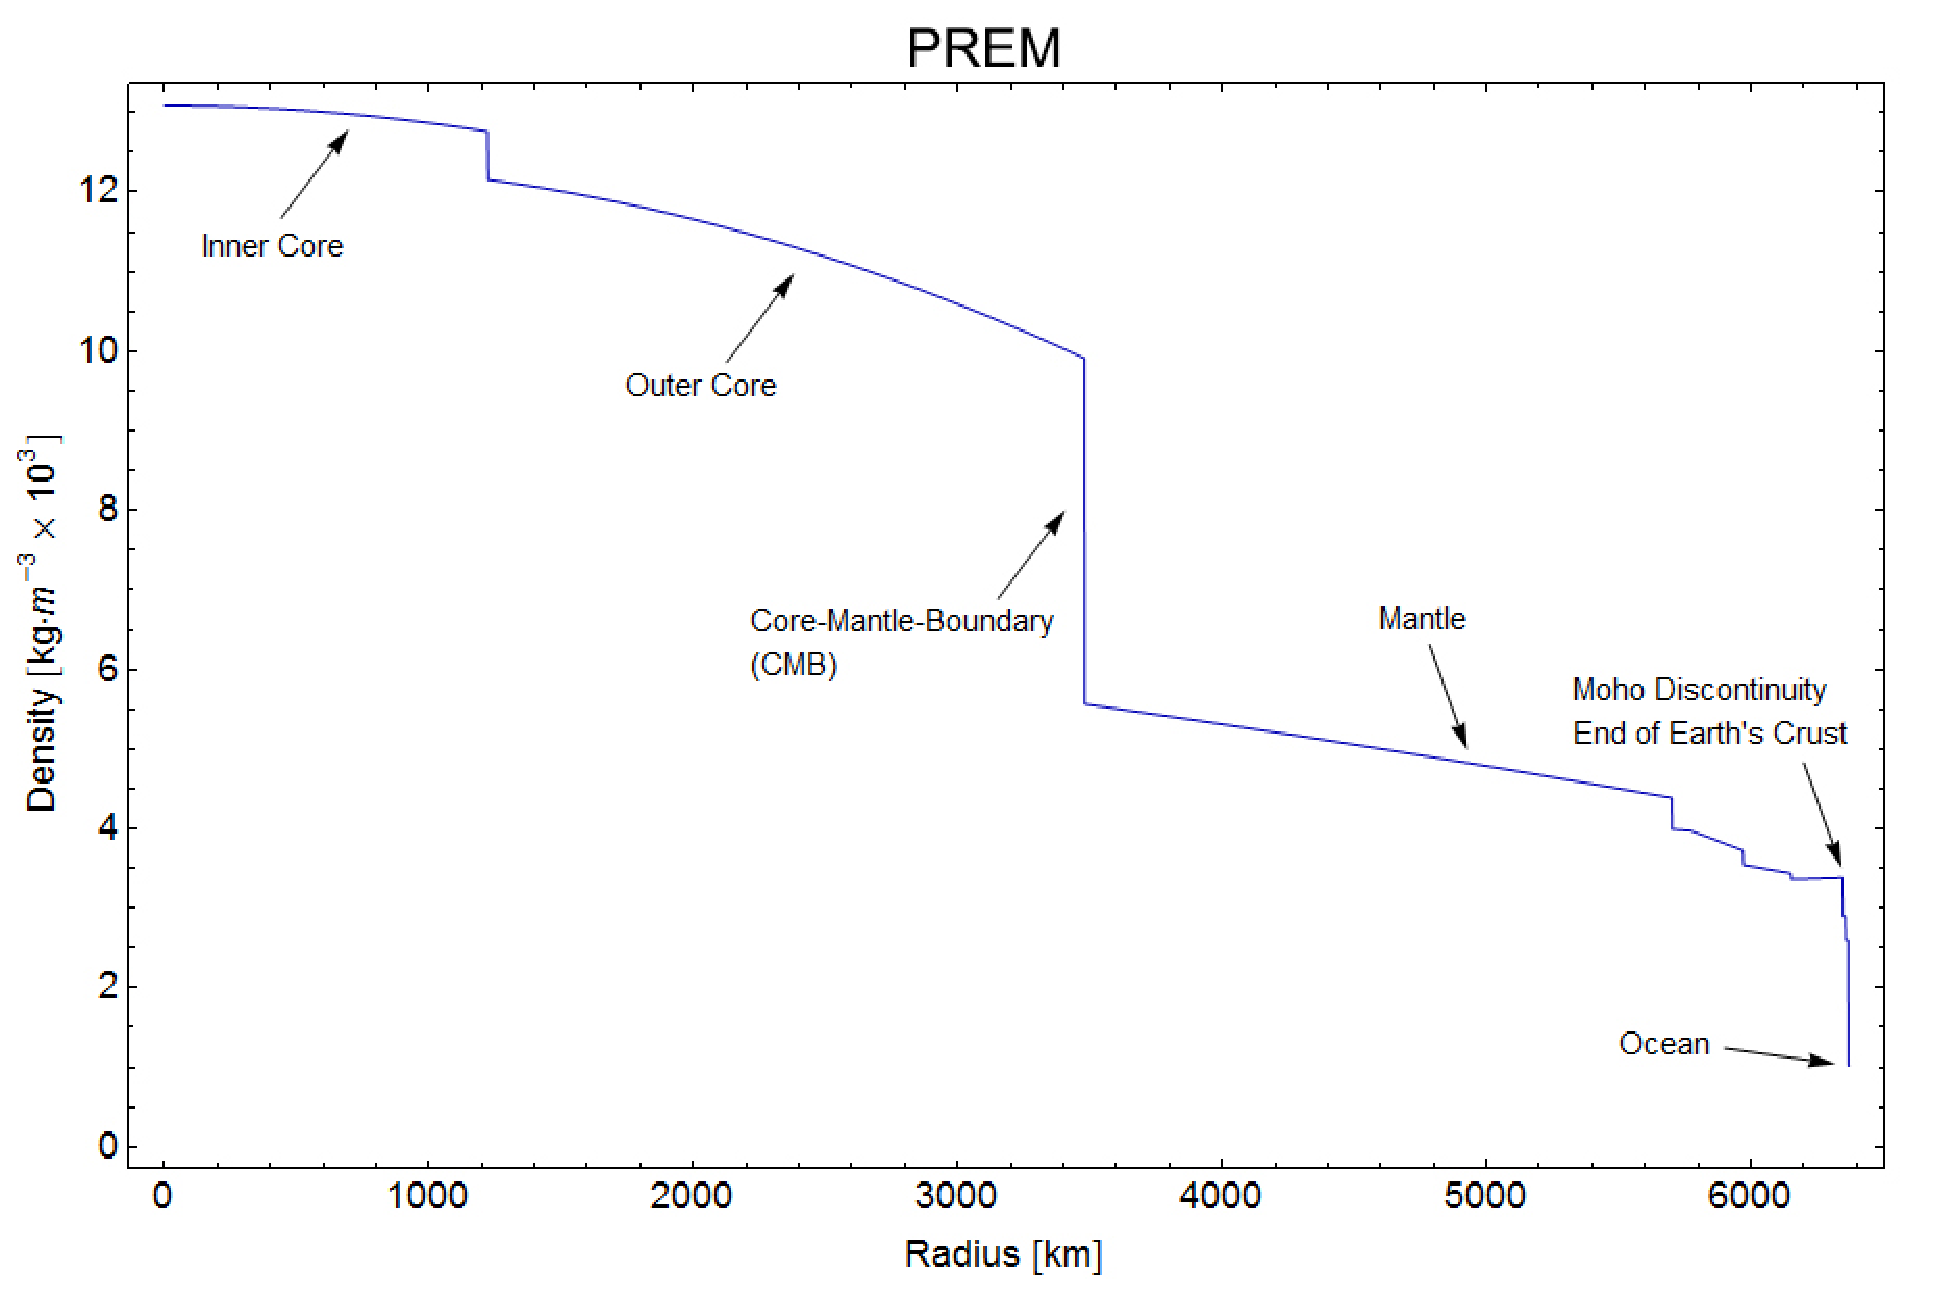
\includegraphics[width=1.0\textwidth]{density.eps}\caption{Density distribution inside the earth according to PREM}
\end{figure}
According to the Preliminary Reference Earth Model, the density inside the Earth increases with the depth. So, we calculated the density as a function of the distance from the center of the earth using the equations for density from the reference model article. 

We know the mass enclosed is equal to:
\begin{equation}
M=\int\limits_0^r\\4 \pi \rho(r) r^{2}\,dr
\end{equation}

where $\rho(r)$ is the density as a function of r (distance from the center of the earth).

From above equations, we get
\begin{equation}
[P(r)-P(r+dr)]A=\frac{GM_{enc}m}{r^2}
\end{equation}
Since the height of the object is very small as compared to the radius of the earth, we can rewrite above equation as:
\begin{equation}
-\frac{dP}{dr}drA=\frac{GM(r)m}{r^{2}}
\end{equation}
We know, $Adr=V$ ,where 'V' is the volume of the object.
or,
\begin{equation}
-\frac{dP}{dr}=\frac{GM(r)}{r^2} (\frac{m}{V})
\end{equation}
Finally, after integrating above equation from the center to the surface of the earth, we get,
\begin{equation}
P(r)=P(RE)+\int\limits_r^{R_E}\\\frac{GM(r)\rho(r)}{r^2}\,dr
\end{equation}

We can also find the moment of inertia of Earth around its axis of rotation if we have an exact calculation of the density as a function of distance to the center of the earth. Since the interior part of the earth is made up of spherical shells, its rotational inertia can be written as:
\begin{equation}
I=\int\limits_0^{R_E} \\\frac{2}{3}\rho(r)4 \pi r^4 \,dr
\end{equation}

\section{Methods}
It was difficult to calculate the density and the mass enclosed as a function of distance from the center of the earth by hand. So, we preferred the use of Python Programming language since it has the open software named 'scipy' specifically designed for the Mathematics, Science and Engineering purposes.

In order to calculate the pressure inside the earth, we used the Simpson's 1/3 rule. We needed to integrate the function for finding pressure from surface of the earth to the center of the earth. So, we broke the interval into a number of small subdivisions. Then we applied Simpson's rule to each subinterval and summed up the results to produce an approximate value for the pressure over entire interval.


\section{Results}
By using the values for Gravitational Constant $(G)=6.67 \times 10^{-11} Nm^{2}kg^{-2}$ , Radius of the earth $(R_E)=6371*10^3 m$ , the value for the pressure at the center of the earth was estimated to be:
\begin{equation}
P_{center}=364.1 \ GPa
\end{equation}
It is almost equal to the realistic value of the pressure at the center of the earth which is about 360 GPa. We also calculated the pressure at every 50 km distance from the surface of the earth and found that the pressure inside the earth increases with the depth. 
\begin{figure}[H]
\centering
\includegraphics[width=1.0\textwidth]{pressure.eps}\caption{Pressure as a function of distance from the center of the earth}
\end{figure}

Finally, by using the values for the density as a function of distance to the center of the earth from the PREM article, we found the value of rotational inertia of the earth which was estimated to be:
\begin{equation}
I=8.02 \times 10^{37} kg m^2
\end{equation}
\end{document}